


\section {Research Motivation}

Historical newspaper archives are of extreme importance for genealogists, scholars and historians. 
There have been extensive studies on text mining from newspapers that deal with clustering newspaper articles into categories\cite{dutta2011learning}, linking similar news stories related to an event \cite{khurdiya2011multi}\cite{shahaf2010connecting}, event extraction from news stories and news story summarization \cite{mckeown2002tracking}.


Historical newspapers can also be used for People Search, for example, to gain information about important people and track the complete timeline of news articles related to them rather than searching for the articles directly. News articles related to an influential person can also be linked to his/her Wikipedia entry so that a user can directly read how, when and where the person had been involved. In fact missing entries can be added to Wikipedia for such influential people across multiple topic categories.
Influential people from historical newspapers can be further studied to find patterns among them and create influential person networks so as to detect themes and learn about entities involved in historical events. This can be done by learning from temporal trends and network structure of connected influential persons and the respective articles they occur in. 


Finding influential persons from historical newspapers, thus,  opens a wide range of possibilities. But the concept of finding influential persons in a newspaper setting is a novel one and has not yet been studied extensively which emphasizes the importance of this research. Using an open source historical news OCR dataset in spite of it being extremely noisy is also another factor which has motivated us to use such a dataset for this research.


\section{Problem Description}
\label{problem}
%%DOUBT: DIFFERENCE BETWEEN AIM AND PROBLEM DESCRIPTION? DO THEY NEED TO BE MENTIONED SEPARATELY?


The goal of this research is to find and rank influential people across multiple topic categories in historical newspaper OCR archives.


%DOUBT:  IS IT OK TO MENTION THESE DETAILS HERE OR THEY SHOULD BE WRITTEN IN RELATED WORK?
The problem of finding influential people in this scenario is a novel one as much of the research work deals with identification of influential nodes in social networks or marketing and diffusion research. This research does not involve finding influential people in terms of their influence on their peers\cite{watts2007influentials} or influence propagation in a social network \cite{kempe2003maximizing} which is how the concept of influence is used in general.   

 An influential person can be defined as ``a person whose actions and opinions strongly influence a course of events". This allows us to link an influential person with a list of articles that he/she occurs in.
 A person might be considered influential  in the newspaper environment if the person gets talked about frequently in news articles. The problem can be also be phrased as identifying and ranking popular people across various categories in the news domain. 
Popularity can be defined in other domains by counting number of votes, tweets, citations, etc. \cite{}but similar measures are not applicable in a newspaper setting where only newspaper articles mentioning multiple people are available.  
 
We divide the the problem of finding influential people into the following subproblems:
\begin{description}
\item [$\bullet $Problem 1] \label{problem:1}: Dealing with a huge dataset consisting of a large number of OCR errors.
\item [$\bullet $Problem 2] \label{2}: Develop an organized structure in order to ease the process of identification of influential people.
\item [$\bullet $Problem 3] \label{3}: Define the criteria for identifying and ranking persons as `influential" in a newspaper environment.
\end{description}
  
Each of the above problems require consideration of the dataset size and characteristics along with the newspaper environment in mind. 



%DOUBT: EITHER WRITE AS WE AIM TO ANSWER THESE QUESTIONS IN THIS RESEARCH OR WE DIVIDE THE PROBLEM INTO THESE SUBPROBLEMS...
%We aim to answer the following questions related to the problem of finding influential people with this research:
%Question 1 : How to deal with OCR data consisting of extremely noisy text for such a task?
%Question 2 : How to develop and use an organized structure for easy identification of influential people?
%Question 3 : Who are `influential persons" in a newspaper scenario and how to rank them?


%DOUBT: NOT SURE WHETHER RESEARCH FRAMEWORK SHOULD COME FIRST OR NOVEL CONTRIBUTION?
\section{Novel Contribution}
We make the following novel contributions for addressing the research problem mentioned in Section ~\ref{problem}:
\begin{enumerate}
\item Develop an evaluation algorithm for measuring the performance of spelling correction preprocessing applied to the dataset consisting of OCR errors.
\item Develop a People Gazetteer; an organized  dictionary of person names and a list of articles in which his name occurs along with the corresponding topic of each article to facilitate identification of influential people.
\item Define an Influential Person Index (IPI) and metrics for its calculation in order to identify and rank influential people.
\end{enumerate}


\section {Research Framework }

We propose the solution framework in Figure 1.1 for the purpose of finding influential people from a historical news repository. Each component of the solution framework is briefly described as follows:

\begin{enumerate}
\item \textbf {Data Gathering}:  
This is the first component of this research and describes the source of gathering data along with data characteristics and statistics. It mentions conversion of page level newspaper images into text through OCR followed by article level segmentation and description of various types of errors in the data. This component is further discussed in Chapter ~\ref{chapter:data description}.

\item \textbf {Data Preprocessing}:
This component describes the preprocessing applied on the news articles dataset. It keys out the process of spelling correction of data in detail with spelling correction algorithm, a novel algorithm for its evaluation and results. This component is further discussed in detail in Chapter ~\ref{chapter:data preprocessing}.

\item \textbf {Development of People Gazetteer}:
This component describes the process of development of people gazetteer which involves Named Entity Recognition in order to find person entities, Topic Detection using LDA to assign topics across the news articles and linking of both to obtain an organized structure. This component is discussed in detail in Chapter ~\ref{chapter:people gazetteer}.

\item \textbf {Influential Person Identification}:
This component defines an ``Influential Person Index" (IPI) that incorporates several criteria for identifying and ranking of ``influential people" across newspaper topics. Details about IPI, ranking and final results with some case studies are discussed in Chapter ~\ref{chapter:influential people detection}.

\end{enumerate}
 
\begin{figure}[h]
\centering
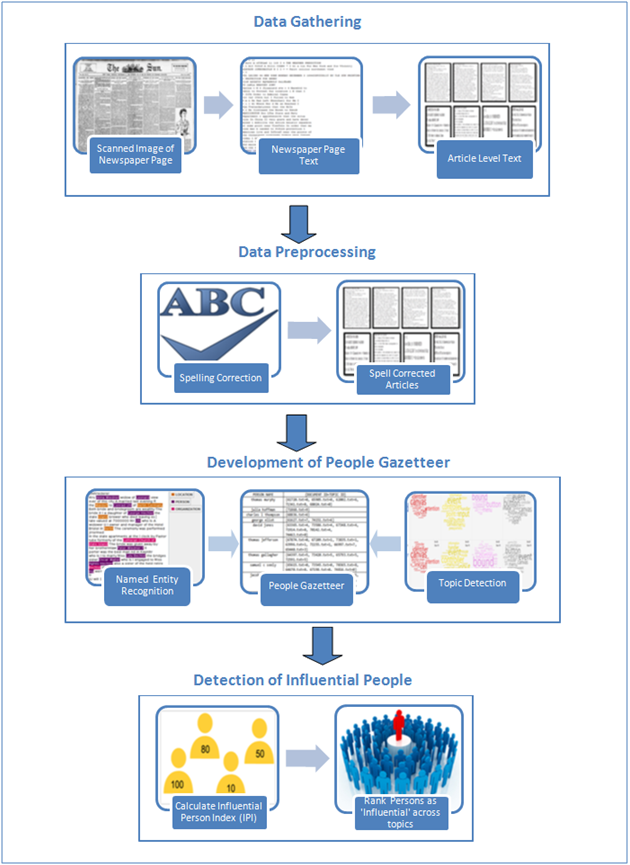
\includegraphics{framework3}
\caption{Research Framework diagram showing components of proposed solution}
\end{figure} 